\documentclass[a4paper,UTF8]{article}
\usepackage{ctex}
\usepackage[margin=1.25in]{geometry}
\usepackage{color}
\usepackage{graphicx}
\usepackage{amssymb}
\usepackage{amsmath}
\usepackage{amsthm}
%\usepackage[thmmarks, amsmath, thref]{ntheorem}
\theoremstyle{definition}
\newtheorem*{solution}{Solution}
\newtheorem*{prove}{Proof}
\usepackage{multirow}
\usepackage{url}
\usepackage{enumerate}
\usepackage{algorithm}
\usepackage{algorithmic}
\usepackage{bm}
\bibliographystyle{plain}

\renewcommand{\algorithmicrequire}{\textbf{Input:}}
\renewcommand{\algorithmicensure}{\textbf{Procedure:}}
\renewcommand\refname{参考文献}

%--

%--
\begin{document}
\title{实验2. 隐马尔科夫模型实践}
\author{MF1733037,刘鑫鑫,\url{xinxliu2014@163.com}}
\maketitle

\section*{综述}
隐马尔科夫模型是一种典型的有向图模型,主要用于时序数据建模。其模型图如下图\ref{fig-1}所示\footnote{图片源于https://cs.nju.edu.cn/wujx/paper/HMM.pdf}。其中$Q_t$是隐马尔科夫模型的隐变量,$O_t$是可观察变量。一个隐马尔科夫模型由参数$\lambda$定义:$\lambda=[A,B,\pi]$。其中A矩阵代表状态转移概率矩阵,其元素$A_{ij}$代表隐变量从状态$s_i$到状态$s_j$的概率;B代表输出观测概率矩阵,其元素$B_{ij} = b_i(o_j)$代表当隐变量的状态为$s_i$时,输出为$o_j$的概率;$\pi$代表初始状态率,$\pi_i$代表模型的初始状态为$s_i$的概率。隐马尔科夫模型满足马尔科夫性质:系统下一时刻的状态仅由当前状态决定,和更久之前的状态无关。
\begin{figure}[htbp]
\centering
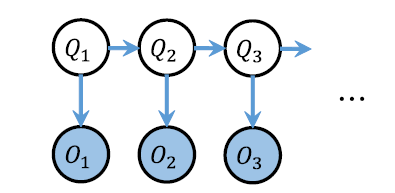
\includegraphics[width=6cm]{1.png}
\caption{隐马尔科夫模型}
\label{fig-1}
\end{figure}

隐马尔科夫模型有三个基本问题\footnote{周志华.机器学习.清华大学出版社,2016},解决这三个问题中的前两个问题便是本次三个实验的主要目的。
\begin{itemize}
\item 给定模型参数$\lambda$和一组观测序列$\bm O$,计算出得到该序列的概率
\item 给定模型参数$\lambda$和一组观测序列$\bm O$,计算出与该观测序列最匹配的隐变量序列$\bm Q$
\item 给定观测序列$\bm O$,如何计算出一个参数模型$\lambda$,使之观测序列为$\bm O$的概率最大

\end{itemize}
其中,解决第一个问题,可以使用本次实验二、三中的forward和backward算法,解决第二个问题,可以使用本次实验一中的Viterbi算法。接下来,笔者将介绍本次任务的三个实验。
\section*{实验一. Viterbi算法}
如前所述,Viterbi算法用于决解第二类问题。该算法实质上是一类动态规划算法。具体来说:给定参数$\lambda = [A,B,\pi]$和观测序列$\bm O=o_{1:T}$,我们需要求的是一组隐变量$\bm Q=Q_{1:T}$(在本次任务代码中用path表示,后面对这两者不加以区分):
\[
\mathop{\arg\max}_{Q_{1:T}}P(Q_{1:T},o_{1:T}|\lambda)
\]
假设隐变量包含N个状态,那么该问题对于给定观测变量$\bm O = o_{1:t}$可以分解为N个子问题:
\[
\delta_t(i)=\max_{Q_{1:t-1}}P(Q_{1:t-1},o_{1:t},Q_t = S_i|\lambda), i = 1,2,\dots,N
\]
那么根据马尔科夫性质,有:
\[
\delta_{t+1}(i) = \max_{1\le j \le N}(\delta_t(j)A_{ji}b_i(o_{t+1}), i = 1,2,\dots, N
\]
由此,得到了关于$\delta$的递推关系式,那么对于N个子问题中,我们需要找到那个最优的子问题$i$,令其为$path_t$,则:
\[
path_t = \mathop{\arg\max}_{1\le j \le N}\delta_t(i)
\]
然后我们需要记录下当在时间t+1时最优状态为$S_i$的时候,时间t对应的那个最优状态:
\[
\phi_{t+1}(i)=\mathop{\arg\max}_{1\le j\le N}(\delta_t(j)A_{ji}b_i(o_{t+1})
\]
进一步简化为:
\[
\phi_{t+1}(i)=\mathop{\arg\max}_{1\le j\le N}(\delta_t(j)A_{ji})
\]

自此,所有的递推式就已经完成,接下来只需加上初始化就可完成算法:
\[
\delta_1(i) = \pi_ib_i(o_1), i = 1,2,\dots,N
\]
\[
\pi_1(i) = 0, i = 1,2,\dots,N
\]

Viterbi算法框架如下算法一所示,具体实现,见本次任务文件“myHMM.py”。
\begin{algorithm}
\label{alg-1}
\caption{Viterbi Algorithm}
\textbf{Input:}\\ 
$\lambda=[A,B,\pi]$\\
$\bm O = o_{1:T}$\\
\textbf{Output:}$path_{1:T}$

\begin{algorithmic}[1]
\STATE initialize $\delta \& \phi$
\FOR{$t \in (2:T-1)$ and $i \in (1:N)$}
\STATE $\delta_{t+1}(i) = \max_{1\le j \le N}(\delta_t(j)A_{ji}b_i(o_{t+1}))$
\STATE $\phi_{t+1}(i)=\mathop{\arg\max}_{1\le j\le N}(\delta_t(j)A_{ji})$
\ENDFOR
\STATE $path_T = \mathop{\arg\max}_{1\le j \le N}\delta_T(i)$
\FOR{$t \in (T-1:1)$}
\STATE $path_t = \phi_{t+1}(path_{t+1})$
\ENDFOR
\end{algorithmic}
\end{algorithm}

\section*{实验二. Forward Algorithm}
前向算法,正如综述中所说,适用于解决第一类问题。即给定模型参数,要求能计算出给定的观测变量$\bm O=o_{1:T}$出现的概率,具体来说,需要求如下联合分布的概率:
\[
P(o_{1:T}|\lambda)
\]
首先根据全概率公式,有:
\[
P(o_{1:T}|\lambda)=\sum^N_{i=1}P(o_{i:T},Q_T=S_i|\lambda)
\]
再根据隐马尔科夫模型的性质,进一步有:
\[
P(o_{1:T}|\lambda)=\sum^N_{i=1}P(o_{i:T-1},Q_T=S_i|\lambda)b_i(o_T)
\]
和Viterbi算法一样,前向算法也是一类动态规划问题。首先分解为N个子问题:
\[
P(o_{i:T-1},Q_T=S_i|\lambda)=\sum_{j=1}^NP(o_{i:T-1},Q_{T-1}=S_i|\lambda)A_{ji}
\]
自此,递推公式已完成。为了表述的简洁,设:
\[
\alpha_t(i)=P(o_{1:t},Q_t = S_i|\lambda)
\]
那么:
\[
\alpha_{t+1}(i)=(\sum_{j=1}^N\alpha_t(j)A_{ji})b_i(o_{t+1})
\]
最后,考虑初始化问题:
\[
\alpha_1(i)=\pi_ib_i(o_1), i = 1,2,\dots,N
\]
最后,forward算法表示如下算法二所示,具体代码见本次任务文件“myHMM.py”。
\begin{algorithm}
\caption{Forward Algorithm}
\textbf{Input:}\\ 
$\lambda=[A,B,\pi]$\\
$\bm O = o_{1:T}$\\
\textbf{Output:}$P(o_{1:T}|\lambda)$

\begin{algorithmic}[1]
\STATE initialize $\alpha_1(i)=\pi_ib_i(o_1), i = 1,2,\dots,N$
\FOR{$t \in (1:T-1)$ and $i \in (1:N)$}
\STATE $\alpha_{t+1}(i)=(\sum_{j=1}^N\alpha_t(j)A_{ji})b_i(o_{t+1})$
\ENDFOR
\STATE $P(o_{1:T}|\lambda)=\sum^N_{i=1}\alpha_T(i)$
\end{algorithmic}
\end{algorithm}
\section*{实验三. Backward Algorithm}
后向算法和前向算法一样,也是用于解决第一类问题,推导过程和前向算法相似,具体来说,为了和前向相区别,这里使用$\beta$来表示递推的那个变量:
\[
\beta_t(i)=P(o_{t+1}:T|Q_t=S_i,\lambda)
\]
那么,往前一步递推:
\[
\beta_t(i) = \sum_{j=1}^NA_{ij}b_j(o_{t+1})\beta_{t+1}(j)
\]
最后的联合分布为:
\[
P(o_{1:T}|\lambda)=\sum_{j=1}^N\pi_ib_i(o_1)\beta_1(i)
\]
考虑初始化:
\[
\beta_T(i) = 1, i = 1,2,\dots,N
\]
那么,算法框架如下,具体实现代码捡本次任务文件“myHMM.py”:
\begin{algorithm}
\caption{Backward Algorithm}
\textbf{Input:}\\ 
$\lambda=[A,B,\pi]$\\
$\bm O = o_{1:T}$\\
\textbf{Output:}$P(o_{1:T}|\lambda)$

\begin{algorithmic}[1]
\STATE initialize $\beta_T(i) = 1, i = 1,2,\dots,N$
\FOR{$t \in (T-1,1)$ and $i \in (1:N)$}
\STATE $\beta_t(i) = \sum_{j=1}^NA_{ij}b_j(o_{t+1})\beta_{t+1}(j)$
\ENDFOR
\STATE $P(o_{1:T}|\lambda)=\sum^N_{i=1}\pi_ib_i(o_1)\beta_1(i)$
\end{algorithmic}
\end{algorithm}

\end{document}